\documentclass{article}
\usepackage[final]{neurips_2018}
\usepackage[utf8]{inputenc} % allow utf-8 input
\usepackage[T1]{fontenc}    % use 8-bit T1 fonts
\usepackage{hyperref}       % hyperlinks
\usepackage{url}            % simple URL typesetting
\usepackage{booktabs}       % professional-quality tables
\usepackage{amsfonts}       % blackboard math symbols
\usepackage{nicefrac}       % compact symbols for 1/2, etc.
\usepackage{microtype}      % microtypography
\usepackage{graphicx}
\graphicspath{{images/}}
\usepackage{caption,subcaption}
\usepackage{array}

\title{Deep Rendering}
\author{Mark Wesley Harris\\
University of Colorado\\
Colorado Springs\\
\texttt{wharris2@uccs.edu} \\
\And
Semwal Sudhanshu\\
University of Colorado\\
Colorado Springs\\
\texttt{ssemwal@uccs.edu} \\
}

\begin{document}

\maketitle

\begin{abstract}
We propose the research and development of new render pipeline
to generate plausible renderings of 3D scenes.
Our proposed work combines current research in deep learning to generate
coarse-to-fine image outputs for portions of the frame being rendered.
These portions can then stitched together to form the final output frame.
The results of our work will give insight into solving the complex problem of
frame prediction without the expense of formal rendering.
Our proposed architecture could also be used to speed up
the animation pipeline itself, by rendering predictions of an animated
scene in real-time based on the data from previously rendered and predicted
frames.
\end{abstract}

\section{Hypothesis}
\label{sec:hypothesis}

\subsection{Research Questions}
\label{subsec:questions}
\begin{enumerate}
\item Is it possible to create a system to generate frames dynamically, based off
past render data and the scene data of previously un-rendered frames?
\item How much resolution and semantic relevance can be expected from the outputs
of such an approach?
\item How do previously rendered frames impact the results of the pipeline given
new inputs?
\item How efficient could the proposed system be, compared to the outputs of
current rendering technologies?
\item Where else might this pipeline be applied?
\end{enumerate}

\subsection{Proposed Methodology}
\label{sec:methodology}
\begin{enumerate}
\item Draft a pipeline that could work in theory based on current research.
\item Apply the latest research in deep image generation to the drafted pipeline.
\item Create training data, including rendered frames (or pieces of frames) with
corresponding binary from the source scene.
\item Evaluate the pipeline on generated and benchmark sources.
\item Compare the results to current state-of-the-art solutions for text-to-image
synthesis and frame prediction.
\end{enumerate}

\section{Introduction}
\label{sec:introduction}
Rendering a 3D scene is time consuming
even for state-of-the-art technology. This is due to the
accumulation of complex computations which occur for each
artifact in the scene and every pixel on the screen. The problem is exacerbated
further for higher resolution renderings wherein millions of objects are present
in the scene, all of which must be processed at rendertime.
We propose using machine learning to assist in the rendering process.
Our proposed system would work alongside current rendering pipelines
to potentially lower the time and resources spent during rendering.
Once trained, we predict the model could also be used to preview small changes in
real-time without re-rendering any parts of the scene, which could have major
implications for real-time rendering technologies such as Augmented and Virtual
Reality.

We propose a study on how relevant scene data in the form of text could be
converted into a corresponding image representative of the rendered frame.
The architecture is built in two stages: a coarse-image generator, focused on
creating global structure; and a fine-image generator, which has the purpose
of up-scaling the output of the first generator and creating a final output.
%of comparable quality and detail as a rendered frame.
We hope to create a baseline that could justify the application of our process
to research in future rendering technologies.
While a deep learning method has not yet been proposed as an aid for rendering
animated sequences, image generation is well researched as a whole.
Here we cover an overview of applicable research,
including an overview of current model architectures and how they could benefit
our proposed work.

\subsection{Generative Adversarial Networks}
\label{subsec:gan}
One highly researched technique is the Generative Adversarial Network (GAN),
first proposed by \cite{generative_adversarial_networks}.
%The GAN was developed as a way to train a model to produce
%more realistic images.
The network is made up of two models,
a generator and a discriminator.
By training both models in tandem,
GANs are able to generate new images that have similar qualities to
those in the dataset which they are trained on.
While the vanilla GAN works fairly well as a random generative model,
\cite{image_transformer} state that GANs
tend to be unstable,
%are ``\dots notoriously unstable``,
and that their outputs
do not reflect the diversity in the training set.
%``\dots fail to reflect the diversity in the training set.''
Recent research, such as \cite{texture_synthesis} and \cite{multiscale_video},
shows that we are able to obtain
higher quality images with more semantic relevance by giving
an algorithm non-random seed data
-- such as a low-quality image or textual description -- to generate from.

\nocite{dcgan}
uses convolutional and convolutional-transpose layers in
the discriminator and generator architectures, respectively.
\cite{pose_guided_image_generation} were successful in using
a variant conditional Deep Convolutional GAN (DCGAN) as their G2 model, and
\cite{unsupervised_learning} employed a DCGAN to
create a generative system for image arithmetic.
%Their results show that GAN architectures could work well
%for generating low-quality images with semantic relevance.
\cite{image_to_image} and \cite{deep_video} used a conditional GAN (cGAN),
which requires a condition image as part of the random input vector.
They found their model worked well in
synthesizing, reconstructing, and colorizing input images.
The Super Resolution GAN (SRGAN), which was first developed through
Single Image Super Resolution (SISR) research,
showed a drastic decrease in loss measurements
other state-of-the-art methods, including Neural Networks and interpolation
%compared to ``NN, bicubic interpolation, and four state-of-the-art methods''
\cite{srgan}.
\cite{semantic_photo} created a system called GANPaint, which allows users to
semantically edit photographs through image representational learning.
\cite{fewer_labels} showed how GANs can be self-supervised to reduce
the amount of labeled data needed during training.
Each of these model architectures improves on the GAN framework to generate
higher-quality images with more relevance to situations in the real world.

\subsection{Non-Adversarial Networks}
\label{subsec:non_adversarial}
GANs are not the only worthwhile image generation algorithms.
A popular alternative in deep image processing is
the Convolutional Neural Network (CNN), which uses filtering operations
in parallel to learn features of input images.
While CNNs excel at feature extraction, researchers have also started to
apply them to the problem of image generation.
\cite{deep_colorization} used a CNN for image colorization, and
\cite{posecnn} developed a CNN to estimate pose information
and object attributes given an input image.
\cite{multiplane} used a fully-convolutional encoder-decoder architecture to
create novel views of a scene using known imagery at learned depths.
One of the most prominent named CNN architectures is PixelCNN,
which uses an input image vector to generate similar output images.
The system was tested by \cite{comparing_simulations} for evaluating simulation
data. \cite{pixelcnn++} provides improvements on the original
PixelCNN architecture, and showed increased efficiency with better outputs.
\cite{parallel_multiscale} also proposed improvements on PixelCNN runtime,
with implications that it could be applied to the problems of
text-to-image synthesis and diverse super-resolution.
%used qualitatively to ``\dots achieve compelling results in text-to-image synthesis and
%video generation, as well as diverse super-resolution from very small images.''

Another class of data translation is the Transformer,
which was first proposed by \cite{attention_need}
as a way to use attention mechanisms more efficiently.
\cite{generative_transformers} explain that Transformers are able to
model an arbitrary number of dependencies in a constant number of layers,
%``\dots model arbitrary dependencies
%in a constant number of layers''
and have proven useful for natural language processing.
In their Sparse Attention architecture, \cite{sparse_transformers} introduced
sparse factorizations on the attention matrix
of a Transformer in order to speed up processing for long sequences of
data.
\cite{image_transformer} performed similar work by using a self-attention
architecture to
generate images with tractable likelihood.
%perform ``\dots a sequence
%modeling formulation of image generation with
%a tractable likelihood.''
%Essentially, they implemented an approximation of the dense attention
%operation by combining several cheaper attention operations.
%The result was a faster and better attention-based architecture
%that could be trained on longer sequences of data 
%\cite{generative_transformers}.
\cite{subscale_pixel} used a network based on Attention as well, which they named
the Subscale Pixel Network (SPN).
Text-to-image generation was notably improved by \cite{attngan}, with their
AttnGAN architecture. The network combines the best of the
generator/discriminator GAN framework with the improvements in
dependency correlation found in Transformers.

\subsection{Data Processing}
\label{subsec:data_processing}
Data from a 3D scene contains countless relationships hidden inside it.
Take for example the problem of representing the
interactions of light on a surface;
what is rendered to the screen completely depends on
the properties of the surface and the amount of light cast onto it.
The addition of realistic lighting properties, such as reflection and refraction,
further complicates the segmentation of scene data.
New research by \cite{3D_capsule_networks} suggests that
Capsule Networks could be more efficient for segmenting shape data
than other neural networks, which
often discard the spatial arrangements inherent in data structures.
%``\dots often discard
%spatial arrangements in data, hence falling short of respecting
%the parts-to-whole relationship, which is critical to explain
%and describe 3D shapes''.
\cite{dynamic_routing} introduced capsule networks (CapsNets) as a powerful
alternative to CNNs. They state that CapsNets learns
a representation of images that is more robust to natural variance.
%``\dots a more equivariant representation of 
%images that is more robust to changes in pose and spatial relationships of
%parts of objects in images'' \cite{transforming_auto_encoders}.
%\cite{dynamic_routing} also argue that, because of the natural variance in
%the representation of data,
%``\dots  CapsNet is moderately robust to small affine transformations of the
%training data.''
The Capsule Network has most recently been extended to 3 dimensions, by
\cite{video_capsule} and \cite{3D_capsule_networks}.
The former used CNs to classify actions in video,
while the latter learned to perform several different manipulations
requiring a greater understanding of the point data as a whole.
The Capsule-GAN proposed by \cite{capsule_synthesis}, \cite{capsgan},
and \cite{capsule_gan},
showed improvements in image generation through dynamic routing.
The researchers stipulate that the emergence of capsules and GANs could improve
frame generation for videos, which is the focus of our proposed work
%``\dots image generation, and plausibly video (frame) generation''
\cite{capsgan}.

\section{Related Work}
\label{sec:related}
We now cover in detail several key sources.
While our scope will not be limited to these sources alone,
they provide the most relevance to our goal. On top of what is mentioned below,
we plan to make use of evaluation metrics, benchmarks, and assessments the
researchers made for their respective projects.

\subsection*{Pose Guided Person Image Generation, 2017}
\nocite{pose_guided_image_generation}
This paper discusses the development of the Pose Guided Person Generation
Network (PG\textsuperscript{2}). PG\textsuperscript{2} contains two stages:
the first is a generative network using several stacked convolutional layers,
which generates an initial course output;
the second is a similar generative network that refines the
result of the previous stage. By combining both of these,
the authors show that it is possible to produce withstanding results of
high similarity to the subject positioned in the target pose
(Figure \ref{fig:pose_guided_image_generation}).
\cite{pose_guided_image_generation} use a U-Net architecture for the generators, 
and a discriminator
similar to that used in the DCGAN created by
\cite{unsupervised_learning}.

The PG\textsuperscript{2} architecture is very relevant to our proposed work,
however there are a few key differences. The ``target pose'' that was used as 
part of the inputs of the first generator is represented in a visual format,
specifically a black and white image with a series of nodes representing the
pose. This standardized representation was also used to mask the reference image,
thereby disregarding data irrelevant to the network.
The generator was thus trained to learn the relationship between two
images -- a target pose and masked input pose. We assert that the complexity of a
scene, which must take into account all objects both
inside and outside the camera's view, cannot be represented in the same format.
%This is evident from the sophistication of current rendering pipelines, which
%make use of ray tracing and Monte Carlo sampling to produce their output.
It is possible that multiple images representing a panoramic view of the scene
could be used, however obtaining these would eliminate the advantages of deep
rendering altogether. To compensate, we propose using semantic scene data in the
form of text. The work of \cite{pose_guided_image_generation}
is still be very useful in determining the
foundation for our proposed network and its components.
%It is unclear whether this text-to-image process will be as fruitful as the
%image-to-image technique employed by Ma et al.

\subsection*{Multi-View Image Generation from a Single-View, 2018}
\nocite{multi_view}
The architecture covered in this paper is similar to that of PG
\textsuperscript{2}
discussed previously; it is also comprised of two generative
networks, and was evaluated in its ability to create a new view of a given pose
(Figure \ref{fig:multi_view}).
\cite{multi_view} argue that it is difficult for basic
Generative Adversarial Networks (GANs) to learn global structures,
which is why they implemented what they
call VariGAN. The VariGAN uses
``\dots variation inference for modeling correct contours and adversarial
learning to fill realistic details.'' The complete architecture
is similar to PG\textsuperscript{2}, but uses primitive word embedding instead of
a standardized representation for inputting conditional data into the coarse
generator. They also only use one conditional discriminator instead of a 
discriminator per generative network.

Although the results of their evaluation were not as good as those with
PG\textsuperscript{2}, \cite{multi_view} include valuable insights for
our proposed work. If nothing else, we will study the differences between the two
generative models. The claimed success of both works provides reassurance for our
proposed network architecture, which relies on conditional data in the form of
text instead of in image format.

\subsection*{Learn, Imagine and Create: Text-to-Image Generation from Prior Knowledge, 2019}
\nocite{leica}
\cite{leica} combine Attention with concepts from GANs to create what they call
LEarn, Imagine and CreAte GAN (LeicaGAN). Similar to the papers discussed
previously, their architecture is comprised of a coarse image generator followed
by a fine image generator. The main difference for the LeicaGAN is their use
of textual-visual co-embedding (TVE) and multiple priors aggregation (MPA)
to further extract semantic meaning from their inputs. \cite{leica} argue that
their network more closely models how the human brain analyzes textual data,
and therefore will have better results in identifying the relationships between
an image and its textual description (Figure \ref{fig:leica}).

The LeicaGAN was not evaluated in the same way as the PG\textsuperscript{2} and
the VariGAN architectures; instead of converting one image to another, they
generate a novel image off of textual input alone. In this sense, the LeicaGAN
is the most relevant research to our proposed work. However, since the results
are more arbitrary, it is possible the network could fail in recognizing the
precise representations and complexities within a scene as a whole.
We propose first using the baseline AttnGAN architecture also used by 
\cite{leica}, and later applying the work from LeicaGAN and other architectures 
to try to improve our results.

\subsection*{Image-to-Image Translation with Conditional Adversarial Networks, 2017}
\nocite{image_to_image}
Isola et al. show that a conditional GAN (cGAN) architecture can be used to
convert from one type of image to another; examples include edges to photograph,
day to night, and black and white to color (Figure \ref{fig:image_to_image}).
The constructed architecture, called
Pix2Pix, uses a U-Net like structure similar to what
\cite{pose_guided_image_generation} developed for
PG\textsuperscript{2}. However, the Pix2Pix discriminator network is modeled off
of the Makovian discriminator created by \cite{markovian},
referred to herein as PatchGAN.
The goal of PatchGAN is to disregard meaning from lower frequency structures,
thereby capturing global phenomenon. \cite{image_to_image}
argue that this discriminator
schema trains the generator to create crisper output images with finer details.

Pix2Pix was evaluated using 9 different tasks. While not all of their
experiments showed improvements from existing technologies, it is noteworthy
in itself that a single network could learn 9 or more types of image conversion.
One of their experiments included converting semantic labels to photographs,
which is particularly relevant to our proposed work.
Pix2Pix falls into the category of image-to-image conversion, which implies that
their achievements may not be directly applicable to our proposed research.
Despite this, we expect that the notable improvements on their discriminator 
architecture could also be applied to our proposed network improve the results
of the generative models.

\subsection*{Blockwise Multi-Order Feature Regression for Real-Time Path Tracing Reconstruction, 2019}
\nocite{path_tracing}
Path tracing is such a computationally intensive process that contemporary
frameworks
``\dots are able to produce only around one path tracing sample per pixel (spp)
at real-time frame rates'' \cite{path_tracing}.
To alleviate this problem, they propose using a
Blockwise Multi-Order Feature Regression (BMFR) algorithm.
As explained, BMFR creates a non-linear fit with respect to the
features of a 1 spp path-traced frame (Figure \ref{fig:path_tracing}).
They also include a preprocessing stage where frame data (including
spacial positions and normals) from previous frames is accumulated to improve
temporal stability of noise. The results of their experiments showed
improvements upon current real-time methods for certain aspects of the image
(such as soft shadows) and also in regards to calculated loss measurements.

Much like the previously discussed research, external data was incorporated
in an image format. The results obtained by \cite{path_tracing}
may serve as a basis
for the argument that image data could in fact be used if it is expressive enough
for training.
While the BMFR algorithm is not an end-to-end solution for us, we may still find
worth in how they up-sampled a low-resolution input frame. In this regard,
we must consider our options for image refinement beyond deep learning.
For now we plan to use a Super Resolution GAN architecture; however, depending on
our final results, BMFR or an alternative algorithm could be
applied to further refine or correct anomalies.

\subsection*{3D Point Capsule Networks, 2019}
\nocite{3D_capsule_networks}
As discussed previously, one of the most prevalent problems in processing raw 3D
scene data is accurately capturing the relationships inherent to the data itself.
\cite{3D_capsule_networks} designed a network architecture to
encapsulate this information into
learned objects of data. Their architecture, called 3D-PointCapsNet,
builds upon the recent research of 2D capsule networks (CNs).
They state that their 3D-PointCapsNet architecture functions as
``\dots an auto-encoder for generic representation
learning in unstructured 3D data''.
The network was trained
to recognize spatial arrangements of 3D point cloud data, as well as perform
numerous tasks such as part segmentation and configuration interpolation
(Figure \ref{fig:3D_capsule_networks}).

This work is promising for the future of 3D shape processing, however its
implications on rendering are yet to be uncovered. Nonetheless, Zhao et al.
proved through their experiments that point capsules could be used to
aid a network in learning the complexities inherent to 3D data, and as such
could be beneficial to our proposed work. A full application of point capsules
as done in 3D-PointCapsNet would disregard the segmented nature of the scene and
likely also the connections between the scene and rendered frame.
We plan to apply their work in discussion on how textual data can be encapsulated
for better learning for our generative networks.

\subsection*{Geometry-Based Next Frame Prediction from Monocular Video, 2017}
\nocite{frame_prediction}
A topic very close to our proposed work is that of frame prediction --
instead of filling in missing frames, the goal of prediction is to create a novel
output based on all previous input data.
\cite{frame_prediction} create a Long Short-Term Memory (LSTM) network
which consumes previous frame information and outputs a depth prediction of the
frame. They then generate the next frame off of the depth prediction, in the same
way as the methods improved upon by \cite{image_to_image},
in applying Pix2Pix to convert one type of image into another
(Figure \ref{fig:frame_prediction}).

The existing results of the LSTM network are close to the
target output, but include gaps where the densities are unknown.
We believe the approach can be generalized to support the premise of
the work by \cite{path_tracing}. and \cite{image_to_image};
it is possible to convert a meaningful semantic representation
of image data into novel image, while withholding the semantic relationship
between source data and rendered frame. \cite{frame_prediction} show that
LSTM architectures would prove useful for temporally related data,
including the source frames we plan to use in our proposed work.

\begin{figure}[h!]
\centering
% PG2
\begin{subfigure}{0.45\textwidth}
\begin{center}
\begin{minipage}[t]{0.855\linewidth}
\begin{centering}
{\includegraphics[width=\linewidth]{pg2_results.png}}
\caption{PG\textsuperscript{2} (\cite{pose_guided_image_generation}).}\label{fig:pose_guided_image_generation}
\end{centering}
\end{minipage}
\end{center}
\end{subfigure}
% BMFR
\begin{subfigure}{0.45\textwidth}
\begin{center}
\begin{minipage}[t]{0.95\linewidth}
\begin{centering}
{\includegraphics[width=\linewidth]{bmfr.png}}
\caption{BMFR Filtering (\cite{path_tracing}).}
\label{fig:path_tracing}
\end{centering}
\end{minipage}
\end{center}
\end{subfigure}
% Leica GAN
\begin{subfigure}{0.45\textwidth}
\begin{center}
\begin{minipage}[t]{0.95\linewidth}
\begin{centering}
{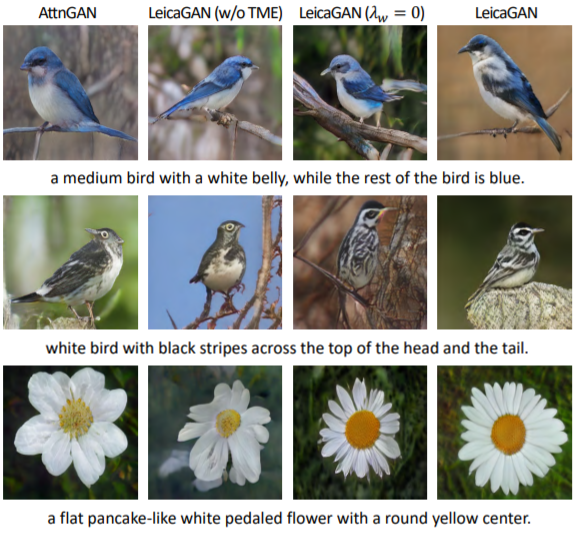
\includegraphics[width=\linewidth]{leicagan.png}}
\caption{LeicaGAN (\cite{leica}).}
\label{fig:leica}
\end{centering}
\end{minipage}
\end{center}
\end{subfigure}
% VariGAN
\begin{subfigure}{0.45\textwidth}
\begin{center}
\begin{minipage}[t]{0.825\linewidth}
\begin{centering}
{\includegraphics[width=\linewidth]{multi_view.png}}
\caption{VariGAN (\cite{multi_view}).}
\label{fig:multi_view}
\end{centering}
\end{minipage}
\end{center}
\end{subfigure}
% Pix2Pix
\begin{subfigure}{0.45\textwidth}
\begin{center}
\begin{minipage}[t]{0.95\linewidth}
\begin{centering}
{\includegraphics[width=\linewidth]{pix2pix.png}}
\caption{Pix2Pix (\cite{image_to_image}).}
\label{fig:image_to_image}
\end{centering}
\end{minipage}
\end{center}
\end{subfigure}
% Capsule Networks
\begin{subfigure}{0.45\textwidth}
\begin{center}
\begin{minipage}[t]{0.925\linewidth}
\begin{centering}
{\includegraphics[width=\linewidth]{capsules.png}}
\caption{3D-PointCapsNet (\cite{3D_capsule_networks}).}
\label{fig:3D_capsule_networks}
\end{centering}
\end{minipage}
\end{center}
\end{subfigure}
% Next frame prediction
\begin{subfigure}{0.45\textwidth}
\begin{center}
\begin{minipage}[t]{0.95\linewidth}
\begin{centering}
{\includegraphics[width=\linewidth]{frame_prediction.png}}
\caption{Frame Prediction \cite{frame_prediction}.}
\label{fig:frame_prediction}
\end{centering}
\end{minipage}
\end{center}
\end{subfigure}
\caption{Graphical references for related work.}
\label{fig:related_work}
\end{figure}

\begin{figure}[h!]
\centering
% Frame samples
\begin{subfigure}{0.45\textwidth}
\begin{center}
\begin{minipage}[t]{0.9\linewidth}
\begin{centering}
{\includegraphics[width=\linewidth]{srgan_frame_samples.png}}
\caption{Generated dataset.}
\label{fig:frame_dataset}
\end{centering}
\end{minipage}
\end{center}
\end{subfigure}
% SRGAN outputs
\begin{subfigure}{0.45\textwidth}
\begin{center}
\begin{minipage}[t]{0.95\linewidth}
\begin{centering}
{\includegraphics[width=\linewidth]{srgan_frame_outputs.png}}
\caption{SRGAN results on input.}
\label{fig:srgan_outputs}
\end{centering}
\end{minipage}
\end{center}
\end{subfigure}
\caption{Initial results for image super resolution using \cite{srgan}.}
\label{fig:initial_results}
\end{figure}

\section{Methodology}
\label{sec:methodology}
Based off of the research referenced above,
we propose an architecture to supplement the rendering process by dynamically
generating plausible frames off of scene data. We refer to this concept as
Deep Rendering. A basic block diagram of the proposed architecture is shown
in Figure \ref{fig:block_diagram}. Here we discuss our proposed approach and
timeline for the research.

\begin{figure}[htbp]
\centerline{\includegraphics[width=8cm]{block_diagram.png}}
\caption{Block diagram for proposed architecture.}
\label{fig:block_diagram}
\end{figure}

\subsection{Approach}
\label{subsec:approach}
The overall structure of our work is
based off of the PG\textsuperscript{2} architecture created by
\cite{pose_guided_image_generation}, as well as the LeicaGAN network
from \cite{leica}. Both architectures obtained remarkable results using
a coarse-to-fine approach in image synthesis, wherein two generative networks
are applied one after the other. We propose to use the same approach;
our Generator I is based off of the Attention GAN model of \cite{attngan},
which should provide a reasonable baseline for image generation;
%which proved to have the best text-to-image capabilities out of all the papers
%surveyed;
Generator II will use the SRGAN by \cite{srgan}, on which we
obtained good results when testing super resolution and anomaly removal
over our generated frameblock dataset.

Depending on the quality of the outputs, a paradigm shift may need to take place.
In this instance, we plan to use the architectures discussed by
\cite{image_transformer}, \cite{sparse_transformers}, and
\cite{3D_capsule_networks} to leverage better
results. We plan to conclude the project with a conference paper ready for
publication. The report will also include the implications of Attention
mechanisms and Capsule Networks -- the two newest architectures to be applied
to deep image generation -- in order to support the completeness
of our work.

\subsection{Initial Results}
\label{subsec:initial}
Our initial work and results are described below.
We first created an animation source file and wrote scripts
to generate training data to be used in our Deep Rendering research.
We also exported textual data pairs for each image, to serve as labels for
the training data. Finally, we worked on the Generator II model, and obtained
good results for anomaly removal. We will next focus on the text-to-image
model for Generator I.

\subsubsection{Data Preprocessing}
\label{subsubsec:data}
In order to generate proper inputs for our proposed system,
a preprocessing phase is necessary for all frames of a given
animated sequence. This process involves selecting portions of each frame
to become a part of the training and test datasets.
We call these portions ``frameblocks'', as they are square sections
of uniform width and height.
By using buffering techniques, we ensure that even the gradual changes in the 
scene are represented in the training data.
Figure \ref{fig:frame_dataset} shows random samples of the training data;
as we required, a majority of the images are unique in correlation to the changes
in the source animation.
%The goal of our first generative model, Generator I, is to produce a crude
%image based on a textual description.
So for every frameblock produced
we must also extract semantic data from the animation source file.
The text-image pair is then fed as input into the generator.
While the exported features may need to be tuned to achieve the best results,
we decided to export name, position, orientation, and property data for each
object represented inside the frameblock. This concludes our preprocessing
for network inputs.

\subsubsection{Generator II}
The second generator, Generator II,
is meant to take the crude, low-quality inputs of the first generative model
and output a higher quality image with believable detail.
Figure \ref{fig:srgan_outputs} shows the output of our SRGAN model trained
on the dataset discussed in Section \ref{subsubsec:data}.
The $\mathbf{\alpha}$ and $\mathbf{\beta}$ parameters control
how much noise and blur was used, respectively.
The results are both analytically and visually promising.
The average accuracy on testing data was 0.84291 for all cases,
which included both strong and weak noise and blur. We are confident that
the SRGAN model will prove capable enough to upsample the crude results of
Generator I.

\subsection{Timeline}
\label{subsec:timeline}
\begin{center}
\def\arraystretch{2.5}
\begin{tabular}{ | m{0.25\textwidth} | m{0.1\textwidth} | m{0.375\textwidth} | m{0.1125\textwidth} | } 
\hline
\textbf{Task} & \textbf{Duration} & \textbf{Description} & \textbf{Status} \\ 
\hline
\hline
Initial project research & 1 month & Foundational research and project planning. & Completed \\
\hline
Data preprocessing & 2 months & Construct a framework for data processing. Create a starting dataset and write documentation on project expectations. & Completed\\
\hline
Create source scene data & 2 weeks & Create a visually-rich animated 3D scene using current animation and rendering technologies. & Completed\\
\hline
Extract scene semantics & 1 month & Extract semantic data for each input frame or portion of the frame. Include scripts for generating the data from the starting dataset in an organized fashion. & Completed \\
\hline
Generator II & 2 months & Research, develop, and test suitable upscaling networks for the proposed second generative model. Compare and document the results. & Completed \\
\hline
Generator I & 3 months & Confirm the work of \cite{leica} in text-to-image generation and apply it to the generated semantics for each frame. & In Progress \\
\hline
Evaluation & 2 weeks & Test the central generative network and determine if further research is required. Alternate options include Attention and/or Capsule Networks. & Pending \\
\hline
Frame reconstruction & 3 months & Reconstruct a frame given the outputs of Generator II. & Not Started \\
\hline
Data collection & 1 month & Collect data from the architecture and compare against current methods and benchmarks. & Not Started\\
\hline
Final documentation & 2 months & Given the final results, complete the thesis and publication write-ups. & Not Started\\
\hline
\end{tabular}
\end{center}

\nocite{pixel_cnn}

\bibliography{proposal}
\bibliographystyle{aaai}

\end{document}
